\section{Subspace Clustering}
The overall idea of subspace clustering is to identify the subspaces that allows better clustering than the full space $\mathcal{S}$. This section discusses two different approaches to subspace clustering, including an analysis of three specific algorithms. All three algorithms follow a bottom-up approach, which requires them to implement the monotonicity property \cite[p.~1:11]{kriegel-2009}, as outlined in Lemma \ref{lem:mono}.

\subsection{Grid-Based approach}
In a grid-based approach, $\mathcal{S}$ is partitioned into an axis-parallel grid structure, where each grid cell forms a axis-aligned, hyper-rectangular \textit{unit}. The number of points within each unit is then counted. This process begins in the 1-dimensional space for each attribute. Units containing a number of points exceeding a predefined \textit{density threshold} are retained as \textit{dense units} (DUs). These DUs are then combined with adjacent ones in the next level (2-dimensional space) to form \textit{candidate dense units} (CDUs). CDUs that meet the density treshold are kept, and this proces continues iteratively. The final set of DUs represent the clusters discovered by the algorithm. These clusters are typically described using minimal representations in the form of \textit{Disjunctive Normal Form} (DNF) expressions, defined by intervals of the attributes. Two algorithms that follows this grid-based approach are CLIQUE and MAFIA.

\subsubsection{CLIQUE}
is the first subspace clustering method to use a grid-based approach. It begins by partitioning $\mathcal{S}$ into equal-sized \textit{windows} (or \textit{units}) with a width of $\varepsilon$ (input parameter). In the 1-dimensional case, DUs are identified by counting the number of points in each window, often using a histogram, as shown in Figure \ref{fig:dense_cells_and_regions}, where each window correspond to a specific \textit{bin} count. For example, if $\varepsilon = 0.2$, CLIQUE identifies 3 DUs in $A_1$ and 4 DUs in $A_2$. The total of 7 DUs in the 1-dimensional space is then used to form CDUs in the 2-dimensional space. Specially, CLIQUE uses the following definition to form CDUs in the $k$-dimensional space:
\begin{definition}\label{def:cdu_clique}
    CDUs in $k$-dimensional space are formed by merging DUs from the $(k-1)$-dimensional space that share the \textit{first} $(k-2)$ attributes.
\end{definition}\todo{måske gøre det klart at det ikke har noget med Apriori at gøre.}
We refer to Definition \ref{def:cdu_clique} as the \textit{first-approach}. Once the CDUs are formed, only those that are actually dense are retained for further processing.

To optimize performance, CLIQUE applies a pruning technique by calculating the \textit{coverage} of subspaces. Subspaces with low coverage--those containing only a small number of points--are pruned to reduce computation time. This method helps manage the potentially large number of CDUs generated by CLIQUE. However, this pruning strategy carries the risk of discarding subspaces that may contain important cluster information.

Once the final DUs are identified, CLIQUE groups them into clusters. A \textit{region} is formed by combining adjacent DUs within a subspace. A \textit{maximal region} is the largest set of connected DUs that cannot be expanded further by adding more adjacent DUs. These maximal regions define the extent of a cluster within the given subspace. For instance, in Figure \ref{fig:dense_cells_and_regions}, two distinct maximal regions, labeled $A$ and $B$, are shown. The minimal representation of the cluster in DNF is: $((0.2 \leq A_1 < 0.6) \land (0.4 \leq A_2 < 0.8)) \lor ((0.4 \leq A_1 < 0.8) \land (0.2 \leq A_2 < 0.6))$.
\begin{figure}[H]
    \centering
    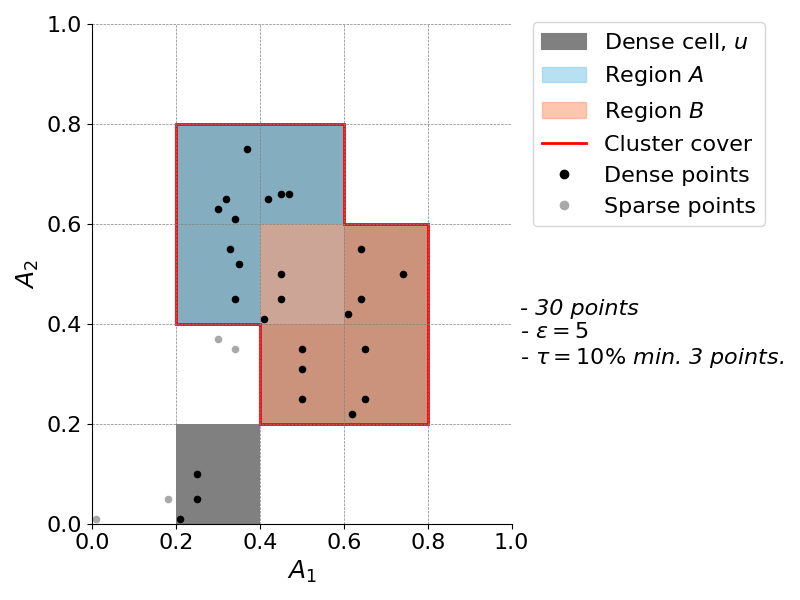
\includegraphics[width=0.55\textwidth]{figures/dense_cells_and_regions.png}
    \caption{2-dimensional space containing 2 overlapping dense regions with 8 DUs in total.}
    \label{fig:dense_cells_and_regions}
    \vspace*{-0.7cm}
\end{figure}

\subsubsection{MAFIA}
extends CLIQUE by introducing the following modifications:
\begin{enumerate}
    \item Automatically determines variable-sized grids based on the data distribution.
    \item Forms CDUs using all combinations of the dimensions present in the DUs.
    \item Eliminates the pruning technique to avoid potential loss of important cluster information, as previously noted.
    \item Attempts to parallelize the clustering process to enhance performance.
\end{enumerate}
Point 1 and 2 will in the following be explained in more detail.

\paragraph{Adaptive Grid Algorithm.}
MAFIA begins by partitioning each attribute into many ($n$-number) of equal-sized windows (default $n = 1000$). Then, from left to right, two adjacent windows are merged if their bin count differ by less than a predefined percentage, $\beta$ (input parameter). A higher $\beta$ value results in more windows being merged, and vice-versa. When two windows are merged, the highest bin count of the two is carried formward for comparison with the next window, rather than summing the counts of the merged pair. Figure \ref{fig:adaptive_grids} illustrates examples before and after applying the adaptive algorithm with different $\alpha$ and $\beta$ values.

After merging, MAFIA determines a \textit{dense-level} for each window, which establishes how many points the window must contain to be considered dense and thus candidate for forming CDUs in higher-dimensional spaces. The dense-level is calculated as: $\text{dense-level} = \frac{\alpha \cdot a\cdot |\mathcal{D}|}{D_i}$, where $a$ is the \textit{size} of the window, $\alpha$ is the \textit{cluster dominance factor} (input parameter), and $D_i$ is the total range of $A_i$. A higher $\alpha$ value leads to a higher dense-level, requiring more points for a window (i.e. unit) to qualify as dense, as shown in Figure \ref{fig:adaptive_grids}.
\begin{figure}[H]
    \vspace*{-0.7cm}
    \hspace*{-0.5cm}
    \centering
    \subfloat[][Before Adaptive.]{%
        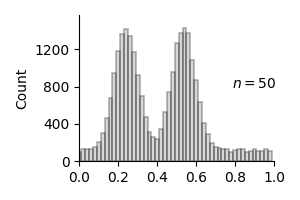
\includegraphics[width=0.26\textwidth]{figures/adaptive_grids/before_adaptive}\label{fig:adaptive_grids_before}}~
    \subfloat[][After Adaptive, $\alpha = 1.5$, $\beta = 20\%$.]{%
        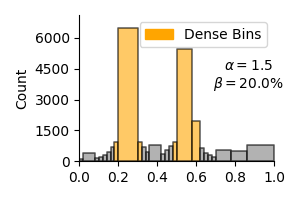
\includegraphics[width=0.26\textwidth]{figures/adaptive_grids/after_adaptive_alpha_1.5_beta_0.2.png}\label{fig:after_adaptive_alpha_1.5_beta_0.2}}~
    \subfloat[][After Adaptive, $\alpha = 2$, $\beta = 20\%$.]{%
        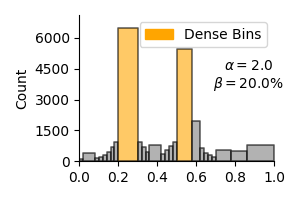
\includegraphics[width=0.26\textwidth]{figures/adaptive_grids/after_adaptive_alpha_2.0_beta_0.2.png}\label{fig:after_adaptive_alpha_2.5_beta_0.2}}~
    \subfloat[][After Adaptive, $\alpha = 2$, $\beta = 30\%$.]{%
        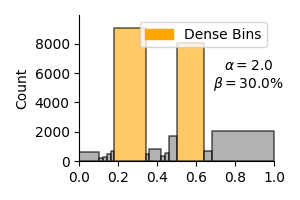
\includegraphics[width=0.26\textwidth]{figures/adaptive_grids/after_adaptive_alpha_2.0_beta_0.3.png}\label{fig:after_adaptive_alpha_2.5_beta_0.3}}~
    \caption{Illustration of the effect of adaptive grids.}
    \label{fig:adaptive_grids}
    \vspace*{-0.7cm}
\end{figure}

\paragraph{CDU Generation in MAFIA.}
MAFIA's approach to generating CDUs differs slightly from that of CLIQUE. MAFIA uses the following definition for forming CDUs in $k$-dimensional space:
\begin{definition}\label{def:cdu_mafia}
    CDUs in $k$-dimensional space are formed by merging DUs from the $(k-1)$-dimensional space that share \textit{any} $(k-2)$ attributes.
\end{definition}
We refer to Definition \ref{def:cdu_mafia} as the \textit{any-approach}. The key distinction between CLIQUE's \textit{first-approach} and MAFIA's any-approach is that MAFIA considers any combination of dimensions shared by the DUs, rather than focusing only on a fixed set of dimensions. Table \ref{tab:cdu} illustrates the advantage of the any-approach. Given 3 DUs in a 4-dimensional space, both CLIQUE and MAFIA would form a 4-dimensional CDU from DU1 and DU2, as they share the first two dimensions. However, only MAFIA would also form a CDU from DU1 and DU3.
\begin{table}[H]
    \vspace*{-0.4cm}
    \centering
    \begin{tabular}{l|c|c|c|}
                        & DU1           & DU2           & DU3           \\ \hline
        Dim. used by DU & $\{1, 2, 3\}$ & $\{1, 2, 4\}$ & $\{2, 3, 4\}$ \\
    \end{tabular}
    \vspace*{0.2cm}
    \caption{Illustration showing the difference between the \textit{first-approach} and \textit{any-approach} with three 3-dimensional DUs.}
    \label{tab:cdu}
    \vspace*{-0.7cm}
\end{table}

While the any-approach can lead to a large number of combinations, potentially resulting in a worst-case time complexity of $O(Ndu^2)$, where $Ndu$ is the number of DUs, MAFIA mitigates this through its adaptive grids, which reduce the number of DUs generated. Although CLIQUE could theoretically implement the any-approach, larger grid sizes would definitely be required to limit the number of DUs, making this less efficient. Note that, the any-approach can lead to duplicate CDUs, which must be eliminated before progressing to higher dimensions.

\subsection{Density-Connected approach}
A drawback of grid-based methods is that clustering quality depends on grid positioning, as illustrated in Figure \ref{fig:dense_cells_and_regions}. Additionally, clusters that deviate from hyper-rectangular shapes are challenging to detect. A potential solution is to use a density-connected algorithm like SUBCLU.

\subsubsection{SUBCLU}
extends the principles of the well-known \textit{DBSCAN} algorithm \cite{dbscan} to higher dimensions. It begins by applying DBSCAN in each 1-dimensional subspace separately, identifying dense regions using two input parameters: $\varepsilon$, which defines the neighborhood radius, and $minPts$, the minimum number of points required for a point to qualify as a \textit{core point}. Points within $\varepsilon$ of a core point, but not dense enough to be core points themselves, are classified as \textit{border points}, while all remaining points are treated as \textit{noise}.

A \textit{density-connected set} consists of core points that are connected through other core points, along with border points that extend the cluster but do not meet the density criteria. These border points are connected to the cluster via core points within their $\varepsilon$-neighborhood. A cluster is thus defined as the union of all density-connected sets, including both core and border points.

After detecting clusters in 1-dimensional subspaces, SUBCLU combines them into higher-dimensional subspaces using the following definition:
\begin{definition}
    Candidate $k$-dimensional subspaces are formed by $(k-1)$-dimensional subspaces that shares any $(k-2)$ dimensions.
\end{definition}

DBSCAN is then reapplied to these candidate subspaces using the same $\varepsilon$ and $minPts$ values to verify whether clusters from lower-dimensional subspaces persist as additional dimensions are considered. To limit the search space, SUBCLU prunes higher-dimensional subspaces based on Lemma \ref{lem:mono}.

Figure \ref{fig:subclu} illustrates an example where SUBCLU identifies a cluster with three points. The algorithm begins by classifying the points in each 1-dimensional subspace and then proceeds to higher-dimensional ones. Note from the figure, that the points may have different classifications accros dimension. For instance, point $d$ is a core point in $A_1$ but a border point in $A_2$.
\begin{figure}[H]
    \vspace*{-0.6cm}
    \centering
    \subfloat[][One 2D cluster found.]{%
        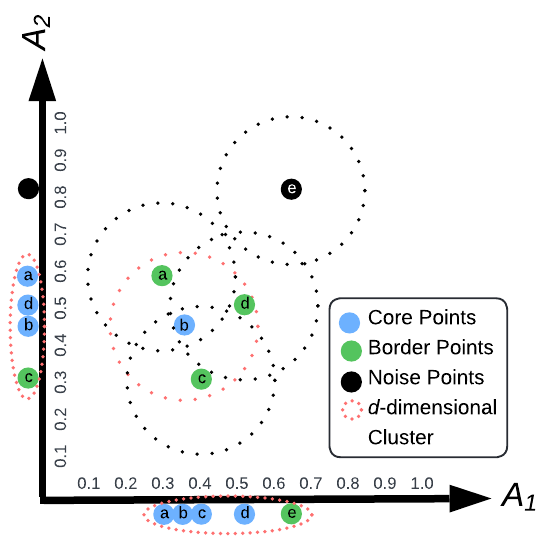
\includegraphics[width=0.36\textwidth]{figures/subclu_cluster.png}\label{fig:subclu_cluster}}~~~~
    \subfloat[][No 2D cluster found after $a$ is moved further up along $A_2$.]{%
        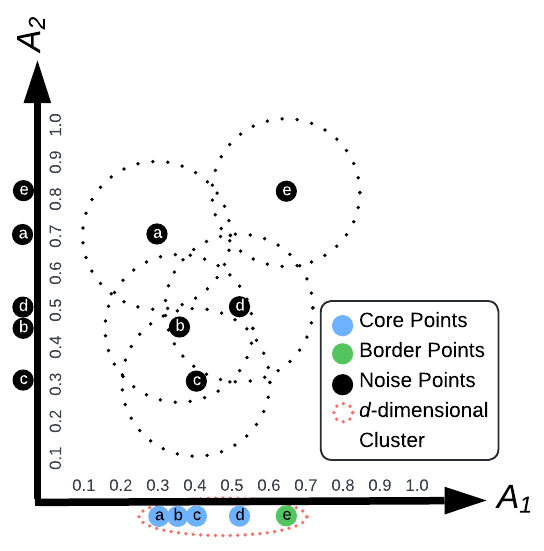
\includegraphics[width=0.36\textwidth]{figures/subclu_no_cluster.png}\label{fig:subclu_no_cluster}}~
    \caption{Illustration of SUBCLU.}
    \label{fig:subclu}
    \vspace*{-0.4cm}
\end{figure}